% 2011 年安徽卷文科第 19 题：多面体 ABEDFC，平面 ABED 与平面 ACFD 垂直，
%   O 在线段 AD 上，OA=1，OD=2，△OAB、△OAC、△ODE、△ODF 都是正三角形。
% 来源 PDF：普通高考/2011/2011安徽文.pdf，SHA-256 af8382bc2cd47a1d5e08bb622275f77ad100aa4f844b5cfd2fd5cd217de58ffc。
% 原页：第 2 页（A3 三栏）第 1 栏中部，书页码 646。
% 重绘依据：照原页——A 在左、D 在右，AD 为被遮挡的虚线；B 在 A 的下方偏右，
%   E 在下方中部、C 在 A 的右上方、F 在正上方偏右；O 在线段 AD 上（图上略偏下标注）。
%   实线：AB、BC、CA、BE、ED、DF、FC、FB、FE；虚线：AD（含 O）、OB、OC、OE、OF。
%   各点位置按原页图形比例摆放，不按真实投影；原页不画顶点圆点。
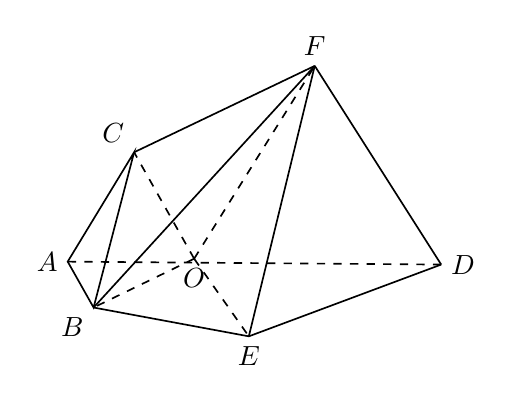
\begin{tikzpicture}[scale=0.62, >=stealth, semithick]
  \coordinate (A) at (0.00,2.20);
  \coordinate (B) at (0.53,1.26);
  \coordinate (C) at (1.36,4.44);
  \coordinate (O) at (2.59,2.26);
  \coordinate (E) at (3.71,0.67);
  \coordinate (D) at (7.65,2.14);
  \coordinate (F) at (5.06,6.21);
  % 可见的棱（实线）
  \draw (A) -- (B) -- (C) -- cycle;
  \draw (B) -- (E) -- (D);
  \draw (F) -- (C);
  \draw (F) -- (B);
  \draw (F) -- (E);
  \draw (F) -- (D);
  % 被遮挡的棱与辅助线（虚线）
  \draw[dashed] (A) -- (D);
  \draw[dashed] (O) -- (B);
  \draw[dashed] (O) -- (C);
  \draw[dashed] (O) -- (E);
  \draw[dashed] (O) -- (F);
  \node at (A) [left]  {$A$};
  \node at (B) [below left] {$B$};
  \node at (C) [above left] {$C$};
  \node at (O) [below] {$O$};
  \node at (D) [right] {$D$};
  \node at (E) [below] {$E$};
  \node at (F) [above] {$F$};
\end{tikzpicture}
